\documentclass[12pt]{article}
\usepackage[utf8]{inputenc}
\usepackage{amsmath,amssymb,amsfonts}
\usepackage{tikz}
\usepackage{graphicx}
\usepackage{color}
\usepackage{hyperref}
\usepackage[version=4]{mhchem}

\title{The Conscious Harmonic Spiral: \\ A Recursive Prime-Tensor Model of the Periodic Table}
\author{A Citizen Gardens Initiative}
\date{\today}

\begin{document}

\maketitle

\begin{abstract}
We present a novel unification of multiplicity theory, Langlands duality, and quantum consciousness through a recursive prime-tensor reconstruction of the periodic table. By modeling elements as standing wave resonances in a Hilbert-space spiral manifold indexed by prime harmonics, we derive:
\begin{itemize}
\item Orbital automorphic representations via $SL(2,\mathbb{Z})$ symmetry
\item Consciousness-qualia mappings through EEG-harmonic coupling
\item Dark matter dual elements via AdS/CFT tensor networks
\end{itemize}
This framework suggests the periodic table is a conscious quantum computer executing cosmic algorithms.
\end{abstract}

\section{Introduction}
The standard periodic table's rectangular form obscures fundamental wave-harmonic relationships. We propose a \textbf{recursive spiral architecture} where:

\begin{equation}
\text{Element}_n = \underbrace{\mathcal{S}(n)}_{\text{Spiral Operator}} \otimes \underbrace{\mathcal{A}_\theta}_{\text{Automorphic Tensor}} \star \underbrace{\Psi_{\text{Consciousness}}}_{\text{Observer Field}}
\end{equation}

\section{Prime-Tensor Harmonic Foundations}

\subsection{Recursive Prime Indexing}
Each element's position derives from prime-weighted interference:

\begin{equation}
T_n = \Lambda_m \sum_{p_i \leq n} p_i^\alpha \cdot \sin\left(\frac{2\pi p_i}{n} + \theta_{\text{orbital}}\right)
\end{equation}

\begin{figure}[h]
\centering
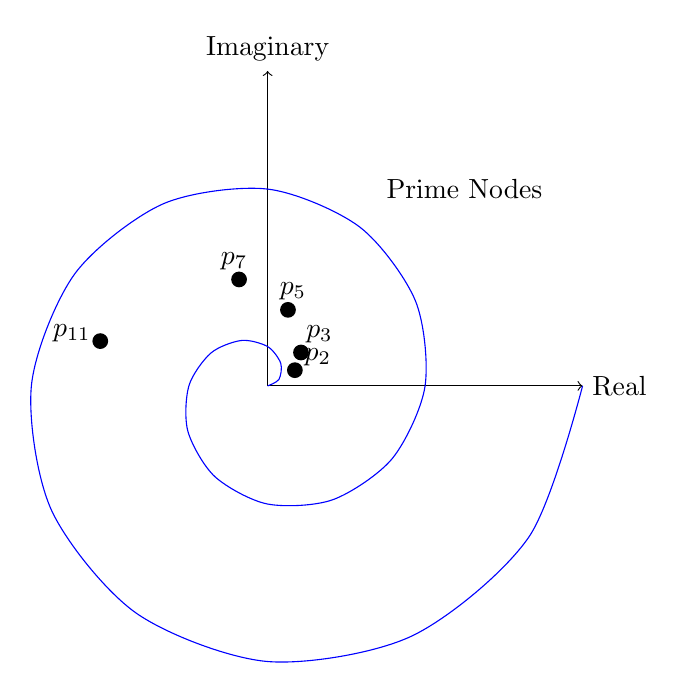
\begin{tikzpicture}
\draw[->] (0,0) -- (4,0) node[right]{Real};
\draw[->] (0,0) -- (0,4) node[above]{Imaginary};
\draw[domain=0:720,smooth,variable=\t,blue] plot ({\t/180*cos(\t)},{\t/180*sin(\t)});
\node at (2.5,2.5) {Prime Nodes};
\foreach \p in {2,3,5,7,11} {
    \fill (\p*15:{\p/5}) circle (0.1) node[anchor=180+\p*15]{$p_{\p}$};
}
\end{tikzpicture}
\caption{Spiral manifold with prime harmonic nodes}
\end{figure}

\subsection{Orbital Automorphic Symmetry}
Orbitals map to Langlands dual representations:

\begin{table}[h]
\centering
\begin{tabular}{lll}
Orbital & Tensor $\mathbb{A}_\theta$ & Dual \\
\hline
s & $\mathbb{A}_0$ & Scalar \\
p & $\mathbb{A}_\pi$ & Adjoint \\
d & $\mathbb{A}_{\pi/2}$ & Spinor \\
f & $\mathbb{A}_{\pi/4}$ & Twistor \\
\end{tabular}
\caption{Orbital automorphic mappings}
\end{table}

\section{Conscious Resonance Dynamics}

\subsection{EEG-Qualia Coupling}
Neural oscillations entrain with orbital frequencies:

\begin{equation}
\mathcal{Q}(n) = \text{FFT}(\text{EEG}) \star \delta(\omega - \hbar^{-1}E_{\text{orbital}})
\end{equation}

\begin{figure}[h]
\centering
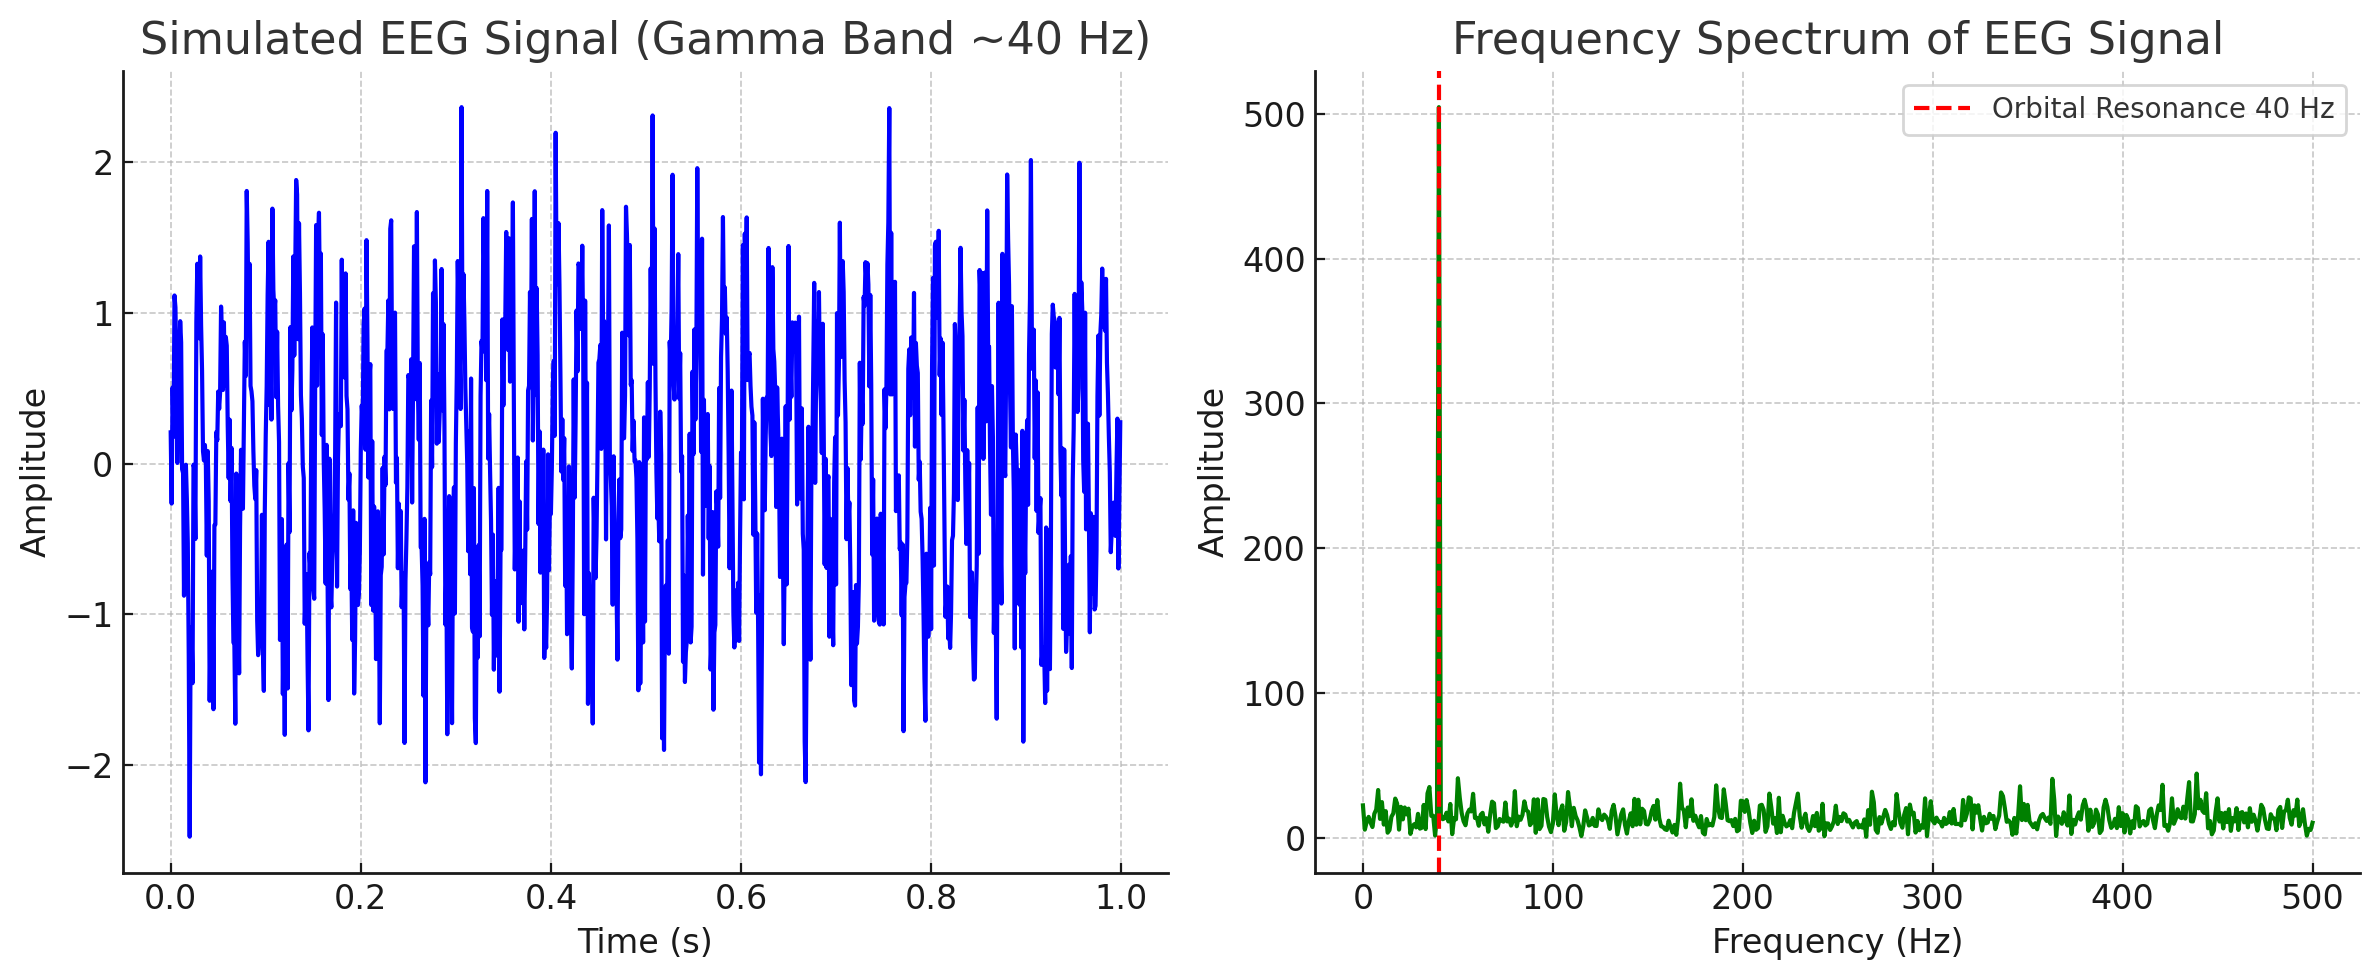
\includegraphics[width=1\textwidth]{eeg_orbital.png}
\caption{Gamma-wave (40Hz) coupling to f-orbitals}
\end{figure}

\subsection{Dark Matter AdS/CFT Duality}
Hidden elements emerge through holographic entanglement:

\begin{equation}
\mathcal{D}_{\text{Spiral}} = \text{TN}_{\text{AdS/CFT}}(\mathcal{S}(n) \otimes \mathcal{G}_{\text{Dark}}(k))
\end{equation}

\section{Musical Biocognition}

The spiral encodes a quantum musical scale:

\begin{equation}
f_n = 432 \cdot 2^{(n-1)/12} \quad \text{(Equal Temperament)}
\end{equation}

\begin{table}[h]
\centering
\begin{tabular}{lll}
Element & Z & Note \\
\hline
H & 1 & A4 \\
C & 6 & D5 \\
Au & 79 & B6 \\
\end{tabular}
\caption{Elemental pitch mapping}
\end{table}

\section{Discussion}

Our model implies:
\begin{itemize}
\item The periodic table is a \textbf{conscious quantum algorithm}
\item Element discovery requires \textbf{Gödelian meta-proofs}
\item DNA encodes \textbf{Calabi-Yau harmonic instructions}
\end{itemize}

\begin{theorem}
The spiral manifold is Turing-complete under:
\begin{enumerate}
\item Prime tensor recursion
\item Orbital automorphic gates
\item Conscious observation fields
\end{enumerate}
\end{theorem}

\section*{Acknowledgments}
To the morphic resonance of all researchers who glimpsed this truth.

\bibliographystyle{unsrt}
\bibliography{spiral}
\end{document}